\section{概要}

\index{HumanInterface}
HumanInterfaceモジュールは,ハードウェアや入力デバイスを利用するための処理系に依存しないインタフェースを提供します.

\KLUDGE ほとんどの場合,HumanInterfaceの機能はFrameworkモジュールを介してアクセスすることになります.
\KLUDGE この場合は,後述するヒューマンインタフェースオブジェクトやデバイスの作成をユーザ自身で行う必要はありません.

\section{HumanInterface SDK}

\index{HISdk}
HumanInterfaceモジュールのすべてのオブジェクトはSDKクラス\texttt{HISdk}によって管理されます.
\texttt{HISdk}クラスは,プログラムの実行を通してただ1つのオブジェクトが存在するシングルトンクラスです.
\texttt{HISdk}オブジェクトを作成するには以下のようにします.
\begin{sourcecode}
HISdkIf* hiSdk = HISdkIf::CreateSdk();
\end{sourcecode}
\KLUDGE 通常この操作はプログラムの初期化時に一度だけ実行します.
\KLUDGE また,Frameworkモジュールを使用する場合はユーザが直接\texttt{HISdk}を作成する必要はありません.

\section{クラス階層とデータ構造}

\begin{figure}[t]
\begin{center}
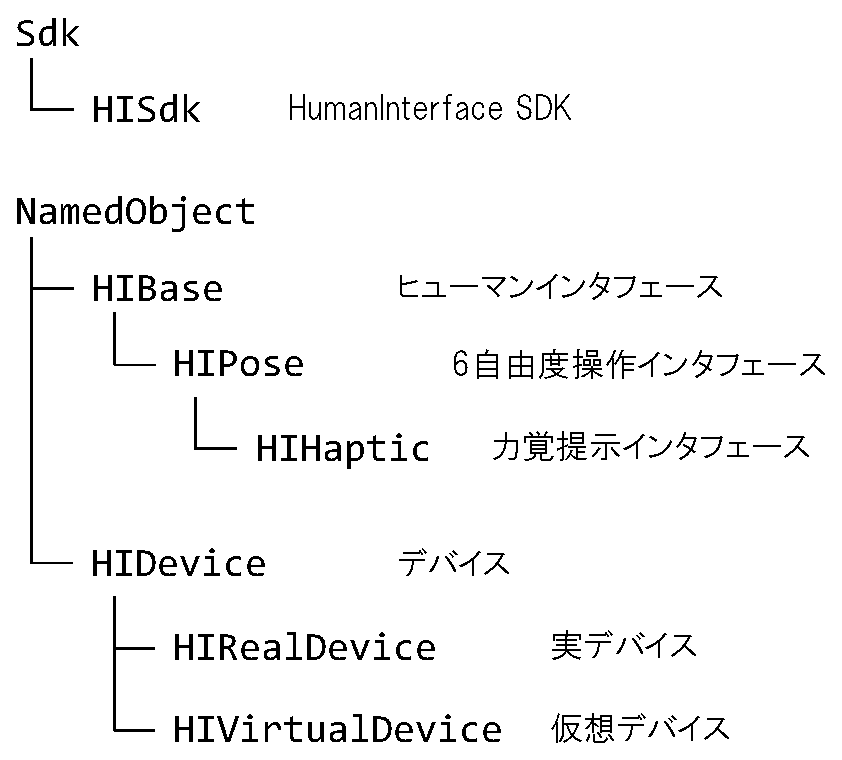
\includegraphics[width=.5\hsize]{fig/hiclass.eps}
\end{center}
\caption{HumanInterface class hierarchy}
\label{fig_hiclass}
\end{figure}

HumanInterfaceモジュールのクラス階層をFig.\,\ref{fig_hiclass}に示します.

\KLUDGE デバイスには実デバイスと仮想デバイスがあります.
\KLUDGE 実デバイスは現実のハードウェアに対応し,例えばWin32マウスやあるメーカのA/D変換ボードを表す実デバイスがあります.
\KLUDGE 一方,仮想デバイスは実デバイスが提供する機能単位を表し,処理系に依存しません.
\KLUDGE 例えば,1つのA/D変換ポートや抽象化されたマウスインタフェースがこれにあたります.
\KLUDGE 基本的に,初期化時を除いてはユーザは実デバイスに触れることはなく,仮想デバイスを通じてそれらの機能を利用することになります.

\KLUDGE ヒューマンインタフェースはデバイスよりも高度で抽象化された操作インタフェースを提供します.


\begin{figure}[t]
\begin{center}
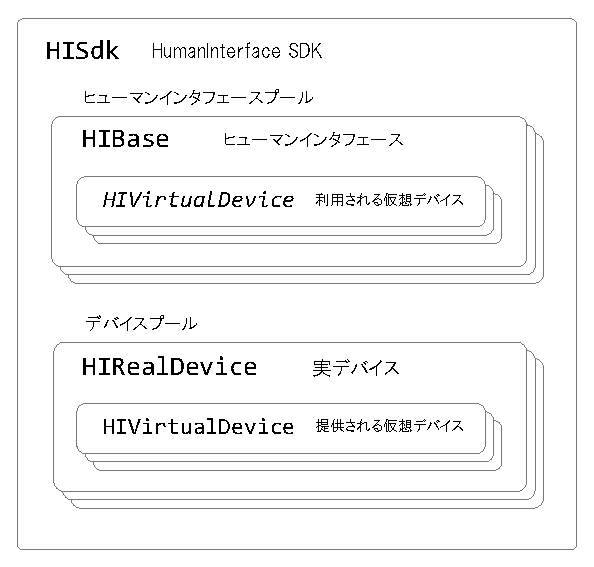
\includegraphics[width=.5\hsize]{fig/humaninterface.eps}
\end{center}
\caption{HumanInterface module data structure}
\label{fig_humaninterface}
\end{figure}

\KLUDGE 次にHumanInterfaceモジュールのデータ構造をFig.\,\ref{fig_humaninterface}に示します.
\texttt{HISdk}オブジェクトはヒューマンインタフェースプールとデバイスプールを持っています.
\KLUDGE デバイスプールとは実デバイスの集まりで,それぞれの実デバイスはその機能をいくつかの仮想デバイスとして外部に提供します.

\KLUDGE デバイスの機能を使うには,
\begin{enumerate}
\item 実デバイスを作成する
\item 実デバイスが提供する仮想デバイスにアクセスする
\end{enumerate}
\KLUDGE という2段階の手順を踏みます.
\KLUDGE 以下にそれに関係する\texttt{HISdk}の関数を紹介します.
\begin{center}
\begin{tabular}{p{.25\hsize}p{.65\hsize}}
\texttt{HISdkIf}																		\\ \midrule
\texttt{HIRealDeviceIf*}	& \texttt{AddRealDevice(const IfInfo* ii, const void* desc = NULL)} \\
\texttt{HIRealDeviceIf*}	& \texttt{FindRealDevice(const char* name)} \\
\texttt{HIRealDeviceIf*}	& \texttt{FindRealDevice(const IfInfo* ii)}
\end{tabular}
\end{center}
\texttt{AddRealDevice}は型情報\texttt{ii}とディスクリプタ\texttt{desc}を指定して実デバイスを作成します.
\texttt{FindRealDevice}は名前か型情報を指定して,既存の実デバイスを検索します.
\KLUDGE たとえば,内部でGLUTを用いるキーボード・マウス実デバイスを取得するには
\begin{sourcecode}
hiSdk->FindRealDevice(DRKeyMouseGLUTIf::GetIfInfoStatic());
\end{sourcecode}
\KLUDGE とします.

\KLUDGE 仮想デバイスを取得および返却する方法には\texttt{HISdk}を介する方法と\texttt{HIRealDevice}を直接呼び出す方法の2通りがあります.
\begin{center}
\begin{tabular}{p{.25\hsize}p{.65\hsize}}
\texttt{HISdkIf}																							\\ \midrule
\texttt{HIVirtualDeviceIf*} & \texttt{RentVirtualDevice(const IfInfo* ii, const char* name, int portNo)}	\\
\texttt{bool}				& \texttt{ReturnVirtualDevice(HIVirtualDeviceIf* dev)}	\\
\end{tabular}
\end{center}
\texttt{RentVirtualDevice}はデバイスプールをスキャンして型情報に合致した最初の仮想デバイスを返します.
\KLUDGE 実デバイスを限定したい場合は\texttt{name}で実デバイス名を指定します.
\KLUDGE また,複数の仮想デバイスを提供する実デバイスもあります.
\KLUDGE この場合はポート番号\texttt{portNo}で取得したい仮想デバイスを指定できます.
\KLUDGE %
\KLUDGE デバイスの競合を防ぐために,一度取得された仮想デバイスは利用中状態になります.
\KLUDGE 利用中のデバイスは新たに取得することはできません.
\KLUDGE 使い終わったデバイスは\texttt{ReturnVirtualDevice}で返却することによって再び取得可能になります.
\begin{center}
\begin{tabular}{p{.25\hsize}p{.65\hsize}}
\texttt{HIRealDeviceIf}																				\\ \midrule
\texttt{HIVirtualDeviceIf*}	& \texttt{Rent(const IfInfo* ii, const char* name, int portNo)}	\\
\texttt{bool}				& \texttt{Return(HIVirtualDeviceIf* dev)}
\end{tabular}
\end{center}
\KLUDGE こちらは実デバイスから直接取得,返却するための関数です.機能は同様です.


\section{実デバイス}

Springheadではいくつかのメーカ製のハードウェアが実デバイスとしてサポートされていますが,
\KLUDGE 処理系に強く依存する部分であるため本ドキュメントの対象外とします.
\KLUDGE 興味のある方はソースコードを見てください.

\section{キーボード・マウス}
\label{sec_hi_keymouse}

\KLUDGE キーボードおよびマウスの機能は包括して1つのクラスとして提供されています.
\KLUDGE キーボード・マウスの仮想デバイスは\texttt{DVKeyMouse}です.
\KLUDGE 実デバイスとしてはWin32 APIを用いる\texttt{DRKeyMouseWin32}とGLUTを用いる\texttt{DRKeyMouseGLUT}があります.
\KLUDGE 提供される機能に多少の差異があるので注意して下さい.

\subsection*{仮想キーコード}

Ascii外の特殊キーには処理系依存のキーコードが割り当てられています.
\KLUDGE この差を吸収するために以下のシンボルが\texttt{DVKeyCode}列挙型で定義されています.

\begin{center}
\begin{tabular}{p{.3\hsize}p{.6\hsize}}
\texttt{DVKeyCode}									\\ \midrule
\texttt{ESC}				& エスケープ			\\
\texttt{F1} - \texttt{F12}	& ファンクションキー	\\
\texttt{LEFT}				& ←					\\
\texttt{UP}					& ↑					\\
\texttt{RIGHT}				& →					\\
\texttt{DOWN}				& ↓					\\
\texttt{PAGE\_UP}			& Page Up				\\
\texttt{PAGE\_DOWN}			& Page Down				\\
\texttt{HOME}				& Home					\\
\texttt{END}				& End					\\
\texttt{INSERT}				& Insert				\\
\end{tabular}
\end{center}

\KLUDGE 必要に応じてシンボルが追加される可能性がありますので,完全なリストはヘッダファイルで確認してください.

\subsection*{コールバック}

\texttt{DVKeyMouse}からのイベントを処理するには\texttt{DVKeyMouseCallback}クラスを継承し,イベントハンドラをオーバライドします.
\texttt{DVKeyMouseCallback}はいくつかのヒューマンインタフェースクラスが継承しているほか,
\KLUDGE 後述するアプリケーションクラス\texttt{FWApp}も継承しています.

\begin{center}
\begin{tabular}{p{.2\hsize}p{.7\hsize}}
\texttt{DVKeyMouseCallback}								\\ \midrule
\texttt{virtual bool} & \texttt{OnMouse(int button, int state, int x, int y)}		\\
\multicolumn{2}{l}{マウスボタンプッシュ/リリース}	\\
\\
\texttt{virtual bool} & \texttt{OnDoubleClick(int button, int x, int y)}			\\
\multicolumn{2}{l}{ダブルクリック}	\\
\\
\texttt{virtual bool} & \texttt{OnMouseMove(int button, int x, int y, int zdelta)}	\\
\multicolumn{2}{l}{マウスカーソル移動/マウスホイール回転}	\\
\\
\texttt{virtual bool} & \texttt{OnKey(int state, int key, int x, int y)}			\\
\multicolumn{2}{l}{キープッシュ/リリース}	\\
\end{tabular}
\end{center}

\texttt{OnMouse}はマウスボタンのプッシュあるいはリリースが生じたときに呼び出されます.
\texttt{button}はイベントに関係するマウスボタンおよびいくつかの特殊キーの識別子を保持し,
\KLUDGE その値は\texttt{DVButtonMask}列挙子の値のOR結合で表現されます.
\texttt{state}はマウスボタン状態変化を示し,\texttt{DVButtonSt}列挙子のいずれかの値を持ちます.
\texttt{x},\texttt{y}はイベント生成時のカーソル座標を表します.
\KLUDGE 例として,左ボタンのプッシュイベントを処理するには次のようにします.
\begin{sourcecode}
// inside your class definition ...
virtual bool OnMouse(int button, int state, int x, int y){
    if(button & DVButtonMask::LBUTTON && state == DVButtonSt::DOWN){
        // do something here
    }
}
\end{sourcecode}

\texttt{OnDoubleClick}はマウスボタンのダブルクリックが生じたときに呼ばれます.
\KLUDGE 引数の定義は\texttt{OnMouse}と同様です.

\texttt{OnMouseMove}はマウスカーソルが移動するか,マウスホイールが回転した際に呼ばれます.
\texttt{button}は直前のマウスプッシュイベントにおいて\texttt{OnMouse}に渡されたのと同じ値を持ちます.
\texttt{x}, \texttt{y}は移動後のカーソル座標,\texttt{zdelta}はマウスカーソルの回転量です.

\texttt{OnKey}はキーボードのキーがプッシュされるかリリースされた際に呼ばれます.
\texttt{state}は\texttt{DVKeySt}列挙子の値を持ちます.
\texttt{key}はプッシュあるいはリリースされたキーの仮想キーコードを保持します.

\KLUDGE 以下に関連する列挙子の定義を示します.

\begin{center}
\begin{tabular}{p{.3\hsize}p{.6\hsize}}
\texttt{DVButtonMask}									\\ \midrule
\texttt{LBUTTON}				& 左ボタン				\\
\texttt{RBUTTON}				& 右ボタン				\\
\texttt{MBUTTON}				& 中ボタン				\\
\texttt{SHIFT}					& Shiftキー押し下げ		\\
\texttt{CONTROL}				& Ctrlキー押し下げ		\\
\texttt{ALT}					& Altキー押し下げ		\\
\end{tabular}
\end{center}

\begin{center}
\begin{tabular}{p{.3\hsize}p{.6\hsize}}
\texttt{DVButtonSt}								\\ \midrule
\texttt{DOWN}			& ボタンプッシュ		\\
\texttt{UP}				& ボタンリリース		\\
\end{tabular}
\end{center}

\begin{center}
\begin{tabular}{p{.3\hsize}p{.6\hsize}}
\texttt{DVKeySt}								\\ \midrule
\texttt{PRESSED}		& 押されている			\\
\texttt{TOGGLE\_ON}		& トグルされている		\\
\end{tabular}
\end{center}

\subsection*{APIとして提供される機能}

\KLUDGE 以下に\texttt{DVKeyMouse}の関数を示します.
\begin{center}
\begin{tabular}{p{.1\hsize}p{.8\hsize}}
\texttt{DVKeyMouseIf}																		\\ \midrule
\texttt{void}	& \texttt{AddCallback(DVKeyMouseCallback*)} 	\\
\texttt{void}	& \texttt{RemoveCallback(DVKeyMouseCallback*)} 	\\
\texttt{int}	& \texttt{GetKeyState(int key)}					\\
\texttt{void}	& \texttt{GetMousePosition(int\& x, int\& y, int\& time, int count=0)}
\end{tabular}
\end{center}
\texttt{AddCallback}はコールバッククラスを登録します.
\KLUDGE 一つの仮想デバイスに対して複数個のコールバックを登録できます.
\texttt{RemoveCallback}は登録済のコールバッククラスを解除します.

\texttt{GetKeyState}は\texttt{DVKeyCode}で指定したキーの状態を\texttt{DVKeySt}の値で返します.

\texttt{GetMousePosition}は\texttt{count}ステップ前のマウスカーソルの位置を取得するのに用います.
\KLUDGE ただし\texttt{count}は$0$以上$63$以下でなければなりません.
\texttt{x}, \texttt{y}にカーソル座標が,\texttt{time}にタイムスタンプが格納されます.

\subsection*{サポート状況に関する注意}

\KLUDGE 使用する実デバイスによっては一部の機能が提供されないので注意して下さい.

\texttt{OnMouseMove}においてマウスホイールの回転量を取得するには,
\KLUDGE 実デバイスとして\texttt{DRKeyMouseWin32}を使用するか,
freeglutとリンクしてビルドしたSpringhead上で\texttt{DRKeyMouseGLUT}を使用する必要があります.

\texttt{OnKey}においてキーのトグル状態を取得するには
\KLUDGE 実デバイスとして\texttt{DRKeyMouseWin32}を使用する必要があります.

\texttt{GetKeyState}は\texttt{DRKeyMouseWin32}でのみサポートされます.

\texttt{GetMousePosition}において,タイムスタンプを取得するには\texttt{DRKeyMouseWin32}を用いる必要があります.

\section{ジョイスティック}

\KLUDGE ジョイスティックの仮想デバイスは\texttt{DVJoyStick}です.
\KLUDGE 実デバイスとしてはGLUTを用いる\texttt{DRJoyStickGLUT}のみがあります.

T.B.D. 

\section{トラックボール}

\begin{figure}[t]
\begin{center}
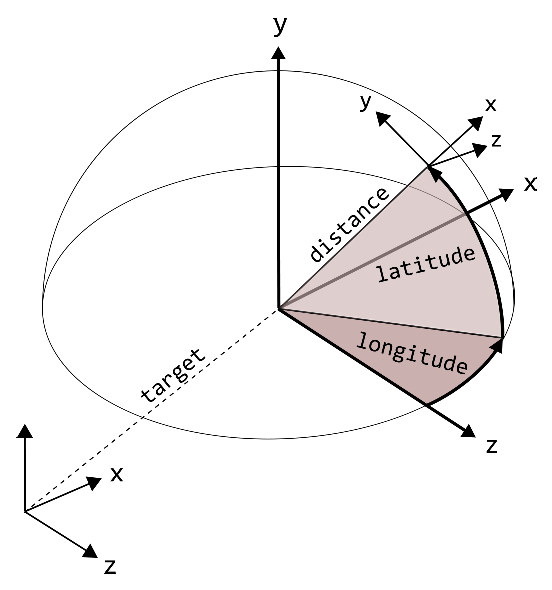
\includegraphics[width=.5\hsize]{fig/hitrackball.eps}
\end{center}
\caption{Trackball}
\label{fig_trackball}
\end{figure}

\KLUDGE トラックボールはキーボード・マウスにより並進・回転の6自由度を入力するヒューマンインタフェースです.
\KLUDGE トラックボールを使うことにより,カメラを注視点まわりに視点変更することができるようになります.

\KLUDGE トラックボールを操作する方法には,APIを直接呼び出す方法と,仮想マウスにコールバック登録する方法の二通りがあります.
\KLUDGE 同様に,トラックボールの状態を取得する方法にもAPI呼び出しとコールバック登録の二通りがあります.
\KLUDGE 仮想マウスとトラックボールおよびユーザプログラムの関係を\figurename\ref{fig_trackball}に示します.


\subsection*{回転中心と回転角度}

\KLUDGE カメラの位置と向きは,注視点,経度角,緯度角および注視点からの距離によって決まります.

\begin{center}
\begin{tabular}{p{.15\hsize}p{.5\hsize}p{.25\hsize}}
\multicolumn{3}{l}{\texttt{HITrackballDesc}}				\\ \midrule
\texttt{Vec3f}	&	\texttt{target}			& 回転中心		\\
\texttt{float}	&	\texttt{longitude}		& 経度[rad]		\\
\texttt{float}	&	\texttt{latitude}		& 緯度[rad]		\\
\texttt{float}	&	\texttt{distance}		& 距離			\\
\end{tabular}
\end{center}

\begin{center}
\begin{tabular}{p{.15\hsize}p{.75\hsize}}
\multicolumn{2}{l}{\texttt{HITrackballIf}}									\\ \midrule
\texttt{Vec3f}	& \texttt{GetTarget()}							\\
\texttt{void} 	& \texttt{SetTarget(Vec3f)}						\\
\texttt{void} 	& \texttt{GetAngle(float\& lon, float\& lat)}	\\
\texttt{void} 	& \texttt{SetAngle(float lon, float lat)}		\\
\texttt{float} 	& \texttt{GetDistance()}						\\
\texttt{void} 	& \texttt{SetDistance(float dist)}				\\
\end{tabular}
\end{center}

\subsection*{範囲指定}

\KLUDGE 以下の機能で角度および距離に範囲制限を加えられます.

\begin{center}
\begin{tabular}{p{.15\hsize}p{.5\hsize}p{.25\hsize}}
\multicolumn{3}{l}{\texttt{HITrackballDesc}}					\\ \midrule
\texttt{Vec2f}	&	\texttt{lonRange}		& 経度範囲			\\
\texttt{Vec2f}	&	\texttt{latRange}		& 緯度範囲			\\
\texttt{Vec2f}	&	\texttt{distRange}		& 距離範囲			\\
\end{tabular}
\end{center}

\begin{center}
\begin{tabular}{p{.15\hsize}p{.75\hsize}}
\multicolumn{2}{l}{\texttt{HITrackballIf}}									\\ \midrule
\texttt{void} 	& \texttt{GetLongitudeRange(float\& rmin, float\& rmax)}	\\
\texttt{void} 	& \texttt{SetLongitudeRange(float rmin, float rmax)}		\\
\texttt{void} 	& \texttt{GetLatitudeRange(float\& rmin, float\& rmax)}		\\
\texttt{void} 	& \texttt{SetLatitudeRange(float rmin, float rmax)}			\\
\texttt{void} 	& \texttt{GetDistanceRange(float\& rmin, float\& rmax)}		\\
\texttt{void} 	& \texttt{SetDistanceRange(float rmin, float rmax)}			\\
\end{tabular}
\end{center}

\subsection*{コールバック登録}

\begin{center}
\begin{tabular}{p{.2\hsize}p{.7\hsize}}
\multicolumn{2}{l}{\texttt{HITrackballIf}}								\\ \midrule
\texttt{DVKeyMouseIf*} 	& \texttt{GetKeyMouse()}						\\
\texttt{void} 			& \texttt{SetKeyMouse(DVKeyMouseIf*)}			\\
\texttt{void} 			& \texttt{SetCallback(HITrackballCallback*)}	\\
\end{tabular}
\end{center}

\KLUDGE トラックボールをマウス操作するには\texttt{DVKeyMouse}クラスにコールバック登録する必要があります.
\KLUDGE コールバック登録するには\texttt{SetKeyMouse},登録先の仮想マウスを取得するには\texttt{GetKeyMouse}を呼びます.

\KLUDGE また,ユーザプログラムがトラックボールにコールバック登録して状態変化に反応できるようにするには,
\texttt{HITrackballCallback}クラスを継承し,\texttt{SetCallback}関数に渡します.
\texttt{HITrackballCallback}は以下の単一の仮想関数を持ちます.
\begin{center}
\begin{tabular}{p{.2\hsize}p{.7\hsize}}
\multicolumn{2}{l}{\texttt{HITrackballCallback}}					\\ \midrule
\texttt{virtual void} 	& \texttt{OnUpdatePose(HITrackballIf* tb)}	\\
\end{tabular}
\end{center}
\texttt{OnUpdatePose}はトラックボールの位置・向きに変化が生じる度に呼ばれます.
\KLUDGE 引数の\texttt{tb}は呼び出し元のトラックボールを示します.

\subsection*{マウスボタン割当て}

\texttt{HITrackball}は内部で\texttt{DVKeyMouseCallback}を継承します.
\texttt{SetKeyMouse}により\texttt{DVKeyMouse}にコールバック登録すると,
\KLUDGE マウスカーソルが移動するたびに\texttt{OnMouseMove}イベントハンドラが呼び出され,トラックボールの内部状態が更新されます.
\KLUDGE マウス移動時のボタン状態に応じてトラックボールのどの状態が変化するかはある程度カスタマイズが可能です.
\KLUDGE 以下に関連する機能を示します.

\begin{center}
\begin{tabular}{p{.15\hsize}p{.35\hsize}p{.4\hsize}}
\multicolumn{3}{l}{\texttt{HITrackballDesc}}		\\ \midrule
\texttt{int}	& \texttt{rotMask}		& 回転操作のボタン割当て		\\
\texttt{int}	& \texttt{zoomMask}		& ズーム操作のボタン割当て		\\
\texttt{int}	& \texttt{trnMask}		& 平行移動操作のボタン割当て	\\
\end{tabular}
\end{center}

\begin{center}
\begin{tabular}{p{.15\hsize}p{.75\hsize}}
\multicolumn{2}{l}{\texttt{HITrackballIf}}			\\ \midrule
\texttt{void} 	& \texttt{SetRotMask(int mask)}		\\
\texttt{void} 	& \texttt{SetZoomMask(int mask)}	\\
\texttt{void} 	& \texttt{SetTrnMask(int mask)}		\\
\end{tabular}
\end{center}

\texttt{rotMask}, \texttt{zoomMask}, \texttt{trnMask}はそれぞれ
\KLUDGE 回転操作,ズーム操作,平行移動操作に割り当てたいマウスボタンに対応する
\texttt{OnMouseMove}の\texttt{button}引数の値を表します.
\KLUDGE 以下に対応関係をまとめます.
\begin{center}
\begin{tabular}{p{.3\hsize}p{.3\hsize}p{.3\hsize}}
\toprule
\KLUDGE マウス移動方向		& \texttt{button}値		& 変化量		\\ \midrule
\KLUDGE 左右				& \texttt{rotMask}		& 経度			\\
\KLUDGE 上下				& \texttt{rotMask}		& 緯度			\\
\KLUDGE 上下				& \texttt{zoomMask}		& 距離			\\
\KLUDGE 左右				& \texttt{trnMask}		& 注視点x座標	\\
\KLUDGE 上下				& \texttt{trnMask}		& 注視点y座標	\\
\bottomrule
\end{tabular}
\end{center}
\KLUDGE デフォルトのボタン割当ては以下の通りです.
\begin{center}
\begin{tabular}{p{.3\hsize}p{.6\hsize}}
\texttt{rotMask}	& \texttt{LBUTTON}					\\
\texttt{zoomMask}	& \texttt{RBUTTON}					\\
\texttt{trnMask}	& \texttt{LBUTTON} + \texttt{ALT}	\\
\end{tabular}
\end{center}
\KLUDGE したがって,左ボタンドラッグで回転操作,右ボタンドラッグでズーム操作,[ALT]キー+左ドラッグで平行移動となります.

\KLUDGE なお,現状ではマウスの移動方向との対応をカスタマイズすることはできません.
\KLUDGE また,マウスホイールの回転とトラックボールを連動させる機能も未実装です.

\subsection*{マウス操作に対する極性と感度}

\KLUDGE マウス移動量と角度変化量,距離変化量との比例係数を下記の機能で設定できます.

\begin{center}
\begin{tabular}{p{.15\hsize}p{.35\hsize}p{.4\hsize}}
\multicolumn{3}{l}{\texttt{HITrackballDesc}}							\\ \midrule
\texttt{float}	&	\texttt{rotGain}		& 回転ゲイン[rad/pixel]		\\
\texttt{float}	&	\texttt{zoomGain}		& ズームゲイン[rad/pixel]	\\
\texttt{float}	&	\texttt{trnGain}		& 平行移動ゲイン			\\
\end{tabular}
\end{center}

\begin{center}
\begin{tabular}{p{.15\hsize}p{.75\hsize}}
\multicolumn{2}{l}{\texttt{HITrackballIf}}									\\ \midrule
\texttt{float} 	& \texttt{GetRotGain()}			\\
\texttt{void} 	& \texttt{SetRotGain(float g)}	\\
\texttt{float} 	& \texttt{GetZoomGain()}		\\
\texttt{void} 	& \texttt{SetZoomGain(float g)}	\\
\texttt{float} 	& \texttt{GetTrnGain()}			\\
\texttt{void} 	& \texttt{SetTrnGain(float g)}	\\
\end{tabular}
\end{center}

\subsection*{トラックボールで視点を動かす}

\KLUDGE トラックボールの位置と向きをカメラに反映するには,
\KLUDGE 描画処理の冒頭で以下のようにします.

\begin{sourcecode}
// given GRRenderIf* render
render->SetViewMatrix(trackball->GetAffine().inv());
\end{sourcecode}

\section{Spidar}

Spidarはワイヤ駆動型の3軸・6軸力覚提示ヒューマンインタフェースです.

T.B.D. 


